\documentclass{standalone}
\usepackage{tikz}
\usetikzlibrary{patterns, positioning}


\begin{document}
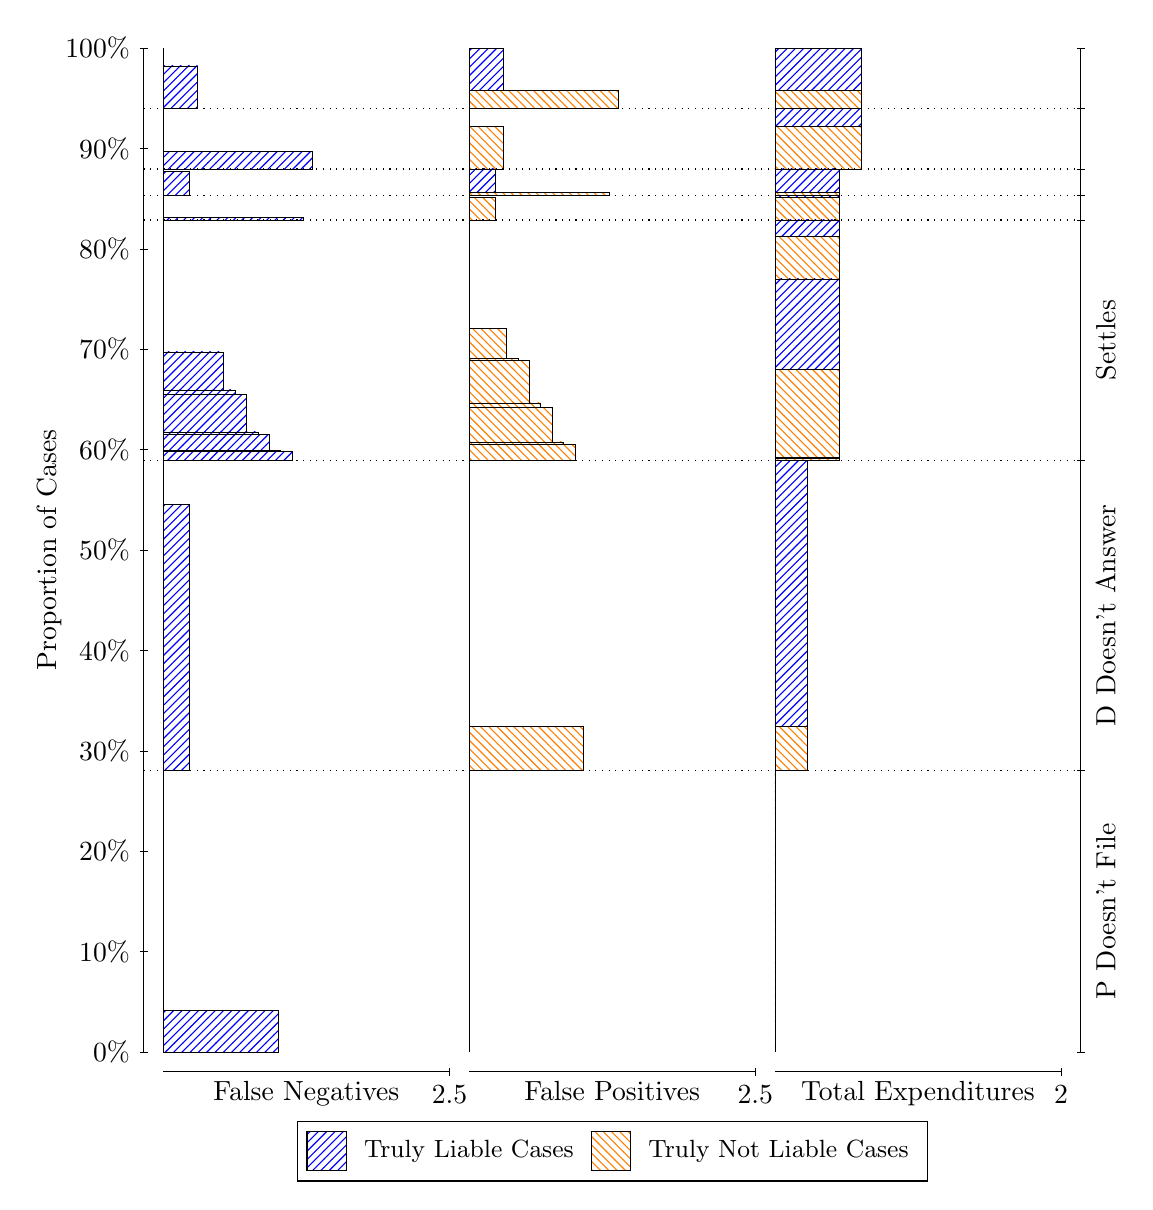
\begin{tikzpicture}
\draw[black, very thin] (1.5,1.75) -- (1.5,14.5);
\node[rotate=90, text=black, anchor=center] at (0.3, 8.125) {Proportion of Cases};
\draw[black, very thin] (1.45,1.75) -- (1.55,1.75);
\node[text=black, anchor=east] at (1.45, 1.75) {0\%};
\draw[black, very thin] (1.45,3.025) -- (1.55,3.025);
\node[text=black, anchor=east] at (1.45, 3.025) {10\%};
\draw[black, very thin] (1.45,4.3) -- (1.55,4.3);
\node[text=black, anchor=east] at (1.45, 4.3) {20\%};
\draw[black, very thin] (1.45,5.575) -- (1.55,5.575);
\node[text=black, anchor=east] at (1.45, 5.575) {30\%};
\draw[black, very thin] (1.45,6.85) -- (1.55,6.85);
\node[text=black, anchor=east] at (1.45, 6.85) {40\%};
\draw[black, very thin] (1.45,8.125) -- (1.55,8.125);
\node[text=black, anchor=east] at (1.45, 8.125) {50\%};
\draw[black, very thin] (1.45,9.4) -- (1.55,9.4);
\node[text=black, anchor=east] at (1.45, 9.4) {60\%};
\draw[black, very thin] (1.45,10.675) -- (1.55,10.675);
\node[text=black, anchor=east] at (1.45, 10.675) {70\%};
\draw[black, very thin] (1.45,11.95) -- (1.55,11.95);
\node[text=black, anchor=east] at (1.45, 11.95) {80\%};
\draw[black, very thin] (1.45,13.225) -- (1.55,13.225);
\node[text=black, anchor=east] at (1.45, 13.225) {90\%};
\draw[black, very thin] (1.45,14.5) -- (1.55,14.5);
\node[text=black, anchor=east] at (1.45, 14.5) {100\%};

\draw[black, very thin] (13.4,1.75) -- (13.4,14.5);
\draw[black, very thin] (13.35,1.75) -- (13.45,1.75);
\node[anchor=west] at (13.35, 1.75) {};
\draw[black, very thin] (13.35,5.3259) -- (13.45,5.3259);
\node[anchor=west] at (13.35, 5.3259) {};
\draw[black, very thin] (13.35,9.2663) -- (13.45,9.2663);
\node[anchor=west] at (13.35, 9.2663) {};
\draw[black, very thin] (13.35,12.316) -- (13.45,12.316);
\node[anchor=west] at (13.35, 12.316) {};
\draw[black, very thin] (13.35,12.632) -- (13.45,12.632);
\node[anchor=west] at (13.35, 12.632) {};
\draw[black, very thin] (13.35,12.964) -- (13.45,12.964);
\node[anchor=west] at (13.35, 12.964) {};
\draw[black, very thin] (13.35,13.733) -- (13.45,13.733);
\node[anchor=west] at (13.35, 13.733) {};
\draw[black, very thin] (13.35,14.5) -- (13.45,14.5);
\node[anchor=west] at (13.35, 14.5) {};

\draw[black, very thin, pattern color=blue, pattern=north east lines] (1.75,1.75) rectangle (3.2033,2.2773);
\draw[black, very thin, pattern color=orange, pattern=north west lines] (1.75,2.2773) rectangle (1.75,5.3259);
\draw[black, very thin, pattern color=blue, pattern=north east lines] (1.75,5.3259) rectangle (2.077,8.7041);
\draw[black, very thin, pattern color=orange, pattern=north west lines] (1.75,8.7041) rectangle (1.75,9.2663);
\draw[black, very thin, pattern color=blue, pattern=north east lines] (1.75,9.2663) rectangle (3.385,9.3816);
\draw[black, very thin, pattern color=blue, pattern=north east lines] (1.75,9.3816) rectangle (3.2397,9.3868);
\draw[black, very thin, pattern color=blue, pattern=north east lines] (1.75,9.3868) rectangle (3.0943,9.5932);
\draw[black, very thin, pattern color=blue, pattern=north east lines] (1.75,9.5932) rectangle (2.949,9.6245);
\draw[black, very thin, pattern color=blue, pattern=north east lines] (1.75,9.6245) rectangle (2.8037,10.098);
\draw[black, very thin, pattern color=blue, pattern=north east lines] (1.75,10.098) rectangle (2.6583,10.159);
\draw[black, very thin, pattern color=blue, pattern=north east lines] (1.75,10.159) rectangle (2.513,10.64);
\draw[black, very thin, pattern color=orange, pattern=north west lines] (1.75,10.64) rectangle (1.75,12.316);
\draw[black, very thin, pattern color=blue, pattern=north east lines] (1.75,12.316) rectangle (3.5303,12.349);
\draw[black, very thin, pattern color=orange, pattern=north west lines] (1.75,12.349) rectangle (1.75,12.632);
\draw[black, very thin, pattern color=blue, pattern=north east lines] (1.75,12.632) rectangle (2.077,12.929);
\draw[black, very thin, pattern color=orange, pattern=north west lines] (1.75,12.929) rectangle (1.75,12.964);
\draw[black, very thin, pattern color=blue, pattern=north east lines] (1.75,12.964) rectangle (3.6393,13.191);
\draw[black, very thin, pattern color=orange, pattern=north west lines] (1.75,13.191) rectangle (1.75,13.733);
\draw[black, very thin, pattern color=blue, pattern=north east lines] (1.75,13.733) rectangle (2.186,14.272);
\draw[black, very thin, pattern color=orange, pattern=north west lines] (1.75,14.272) rectangle (1.75,14.5);
\draw[black, very thin, pattern color=orange, pattern=north west lines] (5.6333,1.75) rectangle (5.6333,4.7986);
\draw[black, very thin, pattern color=blue, pattern=north east lines] (5.6333,4.7986) rectangle (5.6333,5.3259);
\draw[black, very thin, pattern color=orange, pattern=north west lines] (5.6333,5.3259) rectangle (7.0867,5.8881);
\draw[black, very thin, pattern color=blue, pattern=north east lines] (5.6333,5.8881) rectangle (5.6333,9.2663);
\draw[black, very thin, pattern color=orange, pattern=north west lines] (5.6333,9.2663) rectangle (6.9777,9.4689);
\draw[black, very thin, pattern color=orange, pattern=north west lines] (5.6333,9.4689) rectangle (6.8323,9.4974);
\draw[black, very thin, pattern color=orange, pattern=north west lines] (5.6333,9.4974) rectangle (6.687,9.9325);
\draw[black, very thin, pattern color=orange, pattern=north west lines] (5.6333,9.9325) rectangle (6.5417,9.9922);
\draw[black, very thin, pattern color=orange, pattern=north west lines] (5.6333,9.9922) rectangle (6.3963,10.533);
\draw[black, very thin, pattern color=orange, pattern=north west lines] (5.6333,10.533) rectangle (6.251,10.558);
\draw[black, very thin, pattern color=orange, pattern=north west lines] (5.6333,10.558) rectangle (6.1057,10.943);
\draw[black, very thin, pattern color=blue, pattern=north east lines] (5.6333,10.943) rectangle (5.6333,12.316);
\draw[black, very thin, pattern color=orange, pattern=north west lines] (5.6333,12.316) rectangle (5.9603,12.599);
\draw[black, very thin, pattern color=blue, pattern=north east lines] (5.6333,12.599) rectangle (5.6333,12.632);
\draw[black, very thin, pattern color=orange, pattern=north west lines] (5.6333,12.632) rectangle (7.4137,12.668);
\draw[black, very thin, pattern color=blue, pattern=north east lines] (5.6333,12.668) rectangle (5.9603,12.964);
\draw[black, very thin, pattern color=orange, pattern=north west lines] (5.6333,12.964) rectangle (6.0693,13.506);
\draw[black, very thin, pattern color=blue, pattern=north east lines] (5.6333,13.506) rectangle (5.6333,13.733);
\draw[black, very thin, pattern color=orange, pattern=north west lines] (5.6333,13.733) rectangle (7.5227,13.961);
\draw[black, very thin, pattern color=blue, pattern=north east lines] (5.6333,13.961) rectangle (6.0693,14.5);
\draw[black, very thin, pattern color=orange, pattern=north west lines] (9.5167,1.75) rectangle (9.5167,4.7986);
\draw[black, very thin, pattern color=blue, pattern=north east lines] (9.5167,4.7986) rectangle (9.5167,5.3259);
\draw[black, very thin, pattern color=orange, pattern=north west lines] (9.5167,5.3259) rectangle (9.9254,5.8881);
\draw[black, very thin, pattern color=blue, pattern=north east lines] (9.5167,5.8881) rectangle (9.9254,9.2663);
\draw[black, very thin, pattern color=orange, pattern=north west lines] (9.5167,9.2663) rectangle (10.334,9.2867);
\draw[black, very thin, pattern color=blue, pattern=north east lines] (9.5167,9.2867) rectangle (10.334,9.2994);
\draw[black, very thin, pattern color=orange, pattern=north west lines] (9.5167,9.2994) rectangle (10.334,10.415);
\draw[black, very thin, pattern color=blue, pattern=north east lines] (9.5167,10.415) rectangle (10.334,11.569);
\draw[black, very thin, pattern color=orange, pattern=north west lines] (9.5167,11.569) rectangle (10.334,12.11);
\draw[black, very thin, pattern color=blue, pattern=north east lines] (9.5167,12.11) rectangle (10.334,12.316);
\draw[black, very thin, pattern color=orange, pattern=north west lines] (9.5167,12.316) rectangle (10.334,12.599);
\draw[black, very thin, pattern color=blue, pattern=north east lines] (9.5167,12.599) rectangle (10.334,12.632);
\draw[black, very thin, pattern color=orange, pattern=north west lines] (9.5167,12.632) rectangle (10.334,12.668);
\draw[black, very thin, pattern color=blue, pattern=north east lines] (9.5167,12.668) rectangle (10.334,12.964);
\draw[black, very thin, pattern color=orange, pattern=north west lines] (9.5167,12.964) rectangle (10.607,13.506);
\draw[black, very thin, pattern color=blue, pattern=north east lines] (9.5167,13.506) rectangle (10.607,13.733);
\draw[black, very thin, pattern color=orange, pattern=north west lines] (9.5167,13.733) rectangle (10.607,13.961);
\draw[black, very thin, pattern color=blue, pattern=north east lines] (9.5167,13.961) rectangle (10.607,14.5);
\draw[black, dotted] (1.5,5.3259) -- (13.4,5.3259);
\draw[black, dotted] (1.5,9.2663) -- (13.4,9.2663);
\draw[black, dotted] (1.5,12.316) -- (13.4,12.316);
\draw[black, dotted] (1.5,12.632) -- (13.4,12.632);
\draw[black, dotted] (1.5,12.964) -- (13.4,12.964);
\draw[black, dotted] (1.5,13.733) -- (13.4,13.733);
\draw[black, very thin] (1.75,1.5) -- (5.3833,1.5);
\node[text=black, anchor=north] at (3.5667, 1.5) {False Negatives};
\draw[black, very thin] (5.3833,1.45) -- (5.3833,1.55);
\node[text=black, anchor=north] at (5.3833, 1.45) {2.5};

\draw[black, very thin] (5.6333,1.5) -- (9.2667,1.5);
\node[text=black, anchor=north] at (7.45, 1.5) {False Positives};
\draw[black, very thin] (9.2667,1.45) -- (9.2667,1.55);
\node[text=black, anchor=north] at (9.2667, 1.45) {2.5};

\draw[black, very thin] (9.5167,1.5) -- (13.15,1.5);
\node[text=black, anchor=north] at (11.333, 1.5) {Total Expenditures};
\draw[black, very thin] (13.15,1.45) -- (13.15,1.55);
\node[text=black, anchor=north] at (13.15, 1.45) {2};

\node[text=black, centered, rotate=90] at (13.72, 3.538) {P Doesn't File};
\node[text=black, centered, rotate=90] at (13.72, 7.2961) {D Doesn't Answer};
\node[text=black, centered, rotate=90] at (13.72, 10.791) {Settles};





\draw (7.449999999999999,1.5) node[draw=none] (baseCoordinate) {};
\begin{scope}[align=center]
        \matrix[scale=0.5, draw=black, below=0.5cm of baseCoordinate, nodes={draw}, column sep=0.1cm]{
            \node[rectangle, draw, minimum width=0.5cm, minimum height=0.5cm, pattern color=blue, pattern=north east lines] {}; &
            \node[draw=none, font=\small, text=black] (B) {Truly Liable Cases}; &
            \node[rectangle, draw, minimum width=0.5cm, minimum height=0.5cm, pattern color=orange, pattern=north west lines] {}; &
            \node[draw=none, font=\small, text=black] (B) {Truly Not Liable Cases}; \\
            };
\end{scope}

\end{tikzpicture}
\end{document}